\documentclass{article}

\usepackage{graphicx}
\usepackage{epstopdf}
\usepackage{amsmath}
\usepackage{amssymb}

\begin{document}
\title{Asympototic Statistics of Nodal Domains in Quantum Chaotic Billiards in the Semiclassical Limit}
\author{Kyle Konrad\\
  Dartmouth College\\
  Computer Science Department\\
  Advisor: Alex Barnett}
\date{\today}


\section*{Notation}
$N := number of points sampled$

$B := number of basis functions used in vergini method$

$k := wavenumber$

$\Delta x := orthogonal spacing between sampled points$

$\alpha := k \Delta x$

\section*{Introduction}
\subsection*{Motivation}
Quantum Chaos is...

This matters because...

\subsection*{Chaotic Billiards}
\begin{equation}
\label{eq:helmholtz}
(\nabla^{2} - k^{2})u({\bf x}) = 0
\end{equation}


\section*{Methods}
\subsection*{Vergini Method}
Vergini and Saraceno [1995] developed a method of computing extremely high eigenfunctions of chaotic billiards using a scaling method. This method works by creating an approximation of the eigenfunction using a finite number of basis functions. Vergini's scaling method gives provides coefficients for basis functions by solving a linear system whose size is given by the number of basis functions used $B$. We can then perform an arbitrary sampling of the eigenfunction (actually its approximation) by evaluating the basis functions with their coefficients at arbitrary points in the billiard. This sampling is computationally expensive and dominates the time spent solving for coefficients of basis functions as well as counting nodal domains, requiring $M N$ function evaluations.

\subsection*{Counting}
Nodal domains are counted by exploring domains pixel by pixel, marking each pixel as ``counted'' once it has been seen. The searching algorithm usded to explore each domain is a hybrid depth- and breadth-first method where for each pixel, the sign of each neighboring pixel is compared to the sign of the nodal domain and if the sign matches, the neighboring pixel is pushed onto a stack. Exploration then continues by popping a pixel off of the stack. This method was chosen so that the signs of all four neighbors (above, below, right, and left) are known when that pixel is being examined, which is necessary for the adaptive interpolation scheme described below.

Letting $N$ be the number of points the eigenfunction is sampled at, this method has computational complexity $O(N)$. This is because the method performs a fixed number of comparisons for each pixel plus $O(N)$ total comparisons searching for an unseen nodal domain after a nodal domain has been explored. This algorithm uses an array of $N$ integers to store, for each pixel, whether it has been counted, which nodal domain it is in, whether or not it is within the boundary of the billiard, and additional information relating to the interpolation method described below. In addition, this method uses a dynamically sized array as a stack whose size it as most the size of the nodal domain being explored and usually only a fraction of that.

\subsection*{Interpolation}
Because sampling eigenfunctions is expensive, we are limited by $N$ which scales like $\Delta x ^{-2}$. As a consequence of working with relatively coursely sampled grids we encounter scenarios where the connectivity of nodal domains is ambiguous (Fig. \ref{fig:interpolation_sample}).

\begin{figure}[h!]
  \begin{center}
    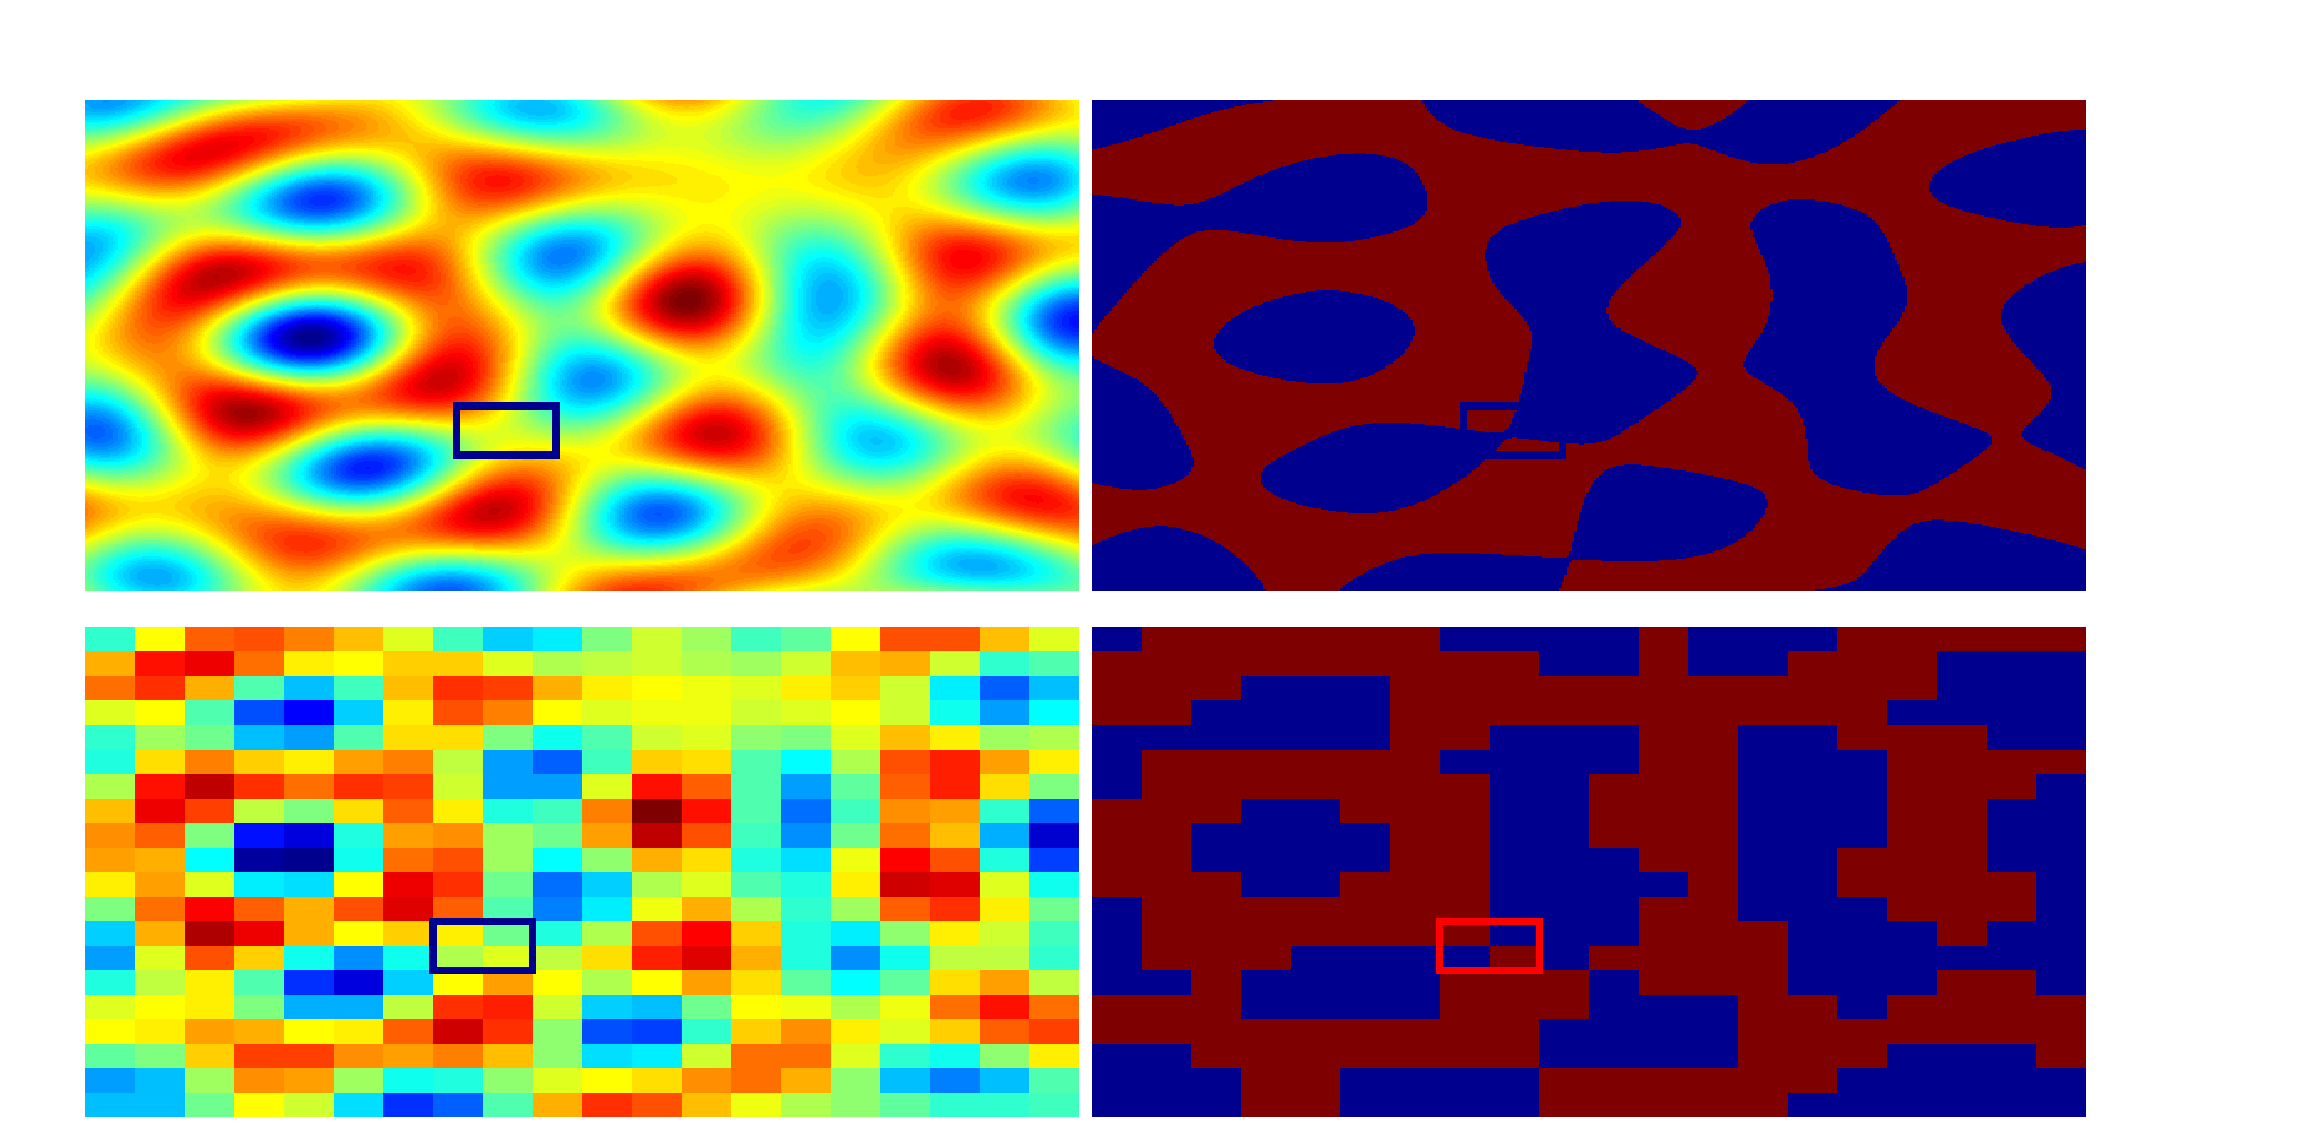
\includegraphics[width=0.75\textwidth]{figures/interpolation/interpolation_sample.eps}
    \caption{An ambiguity in nodal domain connectivity due to coarse sampling. The ambiguous region is shown with a red box. Top left: high resolution image of an eigenfunction; top right: nodal domains of the same eigenfunction; bottom left: low resolution image of the same eigenfunction; bottom right: nodal domains of low resolution eigenfunction}
    \label{fig:interpolation_sample}
  \end{center}
\end{figure}

We resolve such ambiguities by performing an interpolation in the ambigious region. We interpolate with the functions
\begin{equation}
  \xi_{i}(r, \theta)=\begin{cases}
  J_{i}(\alpha r)\sin(i\theta) & \text{if }i>0\\
  J_{i}(\alpha r)\cos(|i|\theta) & \text{if }i<0\\
  J_{i}(\alpha r) & \text{if }i=0
  \end{cases}
\end{equation}
where $J_i(r)$ is a Bessel function (of the first kind)
which form a complete orthonormal basis for solutions of (\ref{eq:helmholtz}). We fix a value $M$ to be the order of the highest order Bessel function, restricting our basis to $\left\{\xi_{i}\right\}_{\vert i \vert \le M}$. We construct a surrogate function
\[
  \tilde{u}({\bf x}) = \sum_{i=-M}^{M} c_{i} \xi_{i}({\bf x})
\]
as a local approximation to the eigenfunction $u({\bf x}$ by fitting the coeffiecients $c_{i} \in \mathbb{R}$ to minimize the error $\Vert u - \tilde{u} \Vert_{2}$. This function can then be sampled at a higher resolution within the region in question. We define the sampling ratio of this surrogate function to the original eigenfunction to be $\rho$.

Because it is only the high resolution sampling of the function we are interested in we can actually skip the step of solving for coefficients and perform the entire computation as a single matrix multiplication my constucting the matrix
\[
U = L H^{+}
\]
Where $L$ is a matrix which performs an evaluation of Bessel functions at low resolution, $H$ performs an evalution of Bessel functions at high resolution and $A^{+}$ denotes the pseudoinverse of $A$. Specifically,
\[
L_{ij} =\begin{cases}
J_{j}({\bf x}_{i}) & \text{for } 
\end{cases}
\]
where ${\bf x}_{i}$ 

\section*{Results}



\end{document}
